De modo a visualizar o "cacho de uvas", foram criados dois predicados \verb|displayOutput/2| e \verb|displayOutput/3|, que apresentam a solução e o puzzle seguido da solução, respetivamente.

A primeira versão do predicado apenas apresenta a solução do problema e é utilizada no predicado \verb|grapesolver/1|.

A segunda versão apresenta tanto o problema como a solução respetiva e é utlizada no predicado \verb|grapegenerator/2|.

\begin{figure}
    \centering
    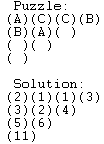
\includegraphics{print.png}
    \caption{Impressão de Resultados}
    \label{fig: results}
\end{figure}